\documentclass{beamer}

\usepackage[utf8]{inputenc}
\usepackage{tikz}
\usepackage{csquotes}
\usepackage{gnuplottex} % [noshell]: do not regenerate gnuplots
\usepackage{booktabs}
\usepackage{xspace, color, svgcolor}
\usepackage{pgfplots}
\usepackage{amsmath}

\usepackage{listings}
\lstset{
  language=python,
  basicstyle=\scriptsize,
}
\usetheme{ODK}
\graphicspath{{Pictures/}}
\usefonttheme[onlymath]{serif}
\newenvironment{smatrix}{\left[\begin{smallmatrix}}{\end{smallmatrix}\right]}
\newcommand{\Z}{\ensuremath{\mathbb{Z}\xspace}}
\newcommand{\Q}{\ensuremath{\mathbb{Q}\xspace}}
\newcommand{\F}{\ensuremath{\mathbb{F}\xspace}}
\usepackage{marvosym}
\newcommand{\GO}[1]{\ensuremath{O(#1)}\xspace}
\newcommand{\SO}[1]{\ensuremath{O\tilde\ (#1)}\xspace}
\newcommand{\thus}{\textcolor{red}{\MVRightarrow{}}\xspace}
\AtBeginSection[]
{
  \begin{frame}<beamer>
    \frametitle{Outline}
    \tableofcontents[currentsection]
  \end{frame}
}

\title[WP 5]{Workpackage 5:\\ High Performance Mathematical Computing}

\author[C. Pernet]{Clément Pernet}

\date[Luxembourg, 2019-10-30]{Luxembourg, October 30, 2019}

\institute[ODK Final project review]{Final OpenDreamKit Project review}

\begin{document}
\maketitle

%%%%%%%%%%%%%%%%%%%%%%%%%%%%%%%%%%%%%%%
\section*{Introduction}

\begin{frame}
  \frametitle{High performance mathematical computing}
  \begin{block}{Mathematical computing}

    %% \begin{columns}
    %%   \begin{column}{.5\textwidth}
    Computing with a large variety of objects
        \begin{itemize}[<+->]
        \item $\Z, \Q, \Z/p\Z, \F_q$, \hfill {\color{blue} $17541718814389012164632$}
        \item Polynomials over $\Z, \Q, \Z/p\Z, \F_q$, \hfill {\color{blue} $\frac{2}{5} x^{3} + x^{2} - \frac{1}{19} x + 2$}
        \item Matrices over $\Z, \Q, \Z/p\Z, \F_q$, \hfill
           {\color{blue} $\begin{smatrix} 27&3&-1\\ 9&0& 2 \end{smatrix} $}
        \item Matrices of polynomials over $\Z, \Q, \Z/p\Z, \F_q$, \hfill
          {\color{blue} $ \begin{smatrix}
            3 x^{2} + 3 & 2 x^{2} + 3 \\4 x^{2} + 1 & x^{2} + 4 x + 4
          \end{smatrix}$}
        \item Tree algebras \hfill
      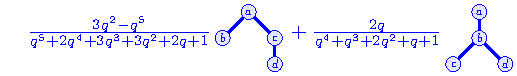
\includegraphics[width=.7\textwidth]{operade}
        \end{itemize}
    %%   \end{column}
    %%   \begin{column}{.45\textwidth}
    %%   \end{column}
    %% \end{columns}

        for applications where all digits matter.

  \end{block}
\end{frame}

\begin{frame}
  \frametitle{High performance mathematical computing}
%  \begin{block}
  \textbf{Need for High performance:} applications where size is crucial:
    \begin{description}
    \item[Experimental maths:] testing conjectures
      \begin{itemize}
      \item larger instances give higher confidence
      \end{itemize}
    \item<2->[Algebraic cryptanalysis:] security = computational difficulty
      \begin{itemize}
      \item key size determined by the largest solvable problem \\
       \begin{minipage}{0.8\textwidth}
        \begin{example}
        {\small Breaking RSA by integer factorization: $n=pq$}.   Last record:
        \begin{itemize}
        \item $n$ of 768 bits
        \item linear algebra in dimension $192\,796\,550$ over $\mathbb{F}_2$ (105Gb)
        \item About 2000 CPU years
        \end{itemize}
      \end{example}\end{minipage}
      \end{itemize}
    \item<3->[3D data analysis, shape recognition:] \
      \begin{itemize}
      \item via persistent homology
      \item large sparse matrices over $\F_2$, \Z
      \end{itemize}
    \end{description}
    
    
    %% \begin{itemize}
    %% \item Decades of development for numerical computations
    %% \item Still at an early development stage for computer algebra
    %% \item Specificites: cannot blindly benefit from numerical HPC experience
    %% \end{itemize}
% \end{block}
\end{frame}
%%%%%%%%%%%%%%%%%%%%%%%%%%%%%%%%%%%%%%%%%%%%%%%%%%%%%%%%%%%%%%%%%
\begin{frame}
  \frametitle{Goal: delivering high performance to maths users}

\uncover<2->{
  \only<1,2>{
    \begin{block}{Harnessing modern hardware $\leadsto$ parallelisation}
  \begin{itemize}
    \item in-core parallelism (SIMD vectorisation)
    \item multi-core parallelism
    \item distributed computing: clusters, cloud
    \end{itemize}
  \end{block}
  }
  
  \only<3>{
    \begin{block}{Languages}
    \begin{itemize}
    \item Computational Maths software uses high level languages (e.g. Python)
    \item High performance delivered by languages close to the metal (C, assembly)
    \end{itemize}
    $\leadsto$ compilation,  automated optimisation
  \end{block}
    \vspace{.5mm}
  }
}


  \begin{center}

    \only<1>{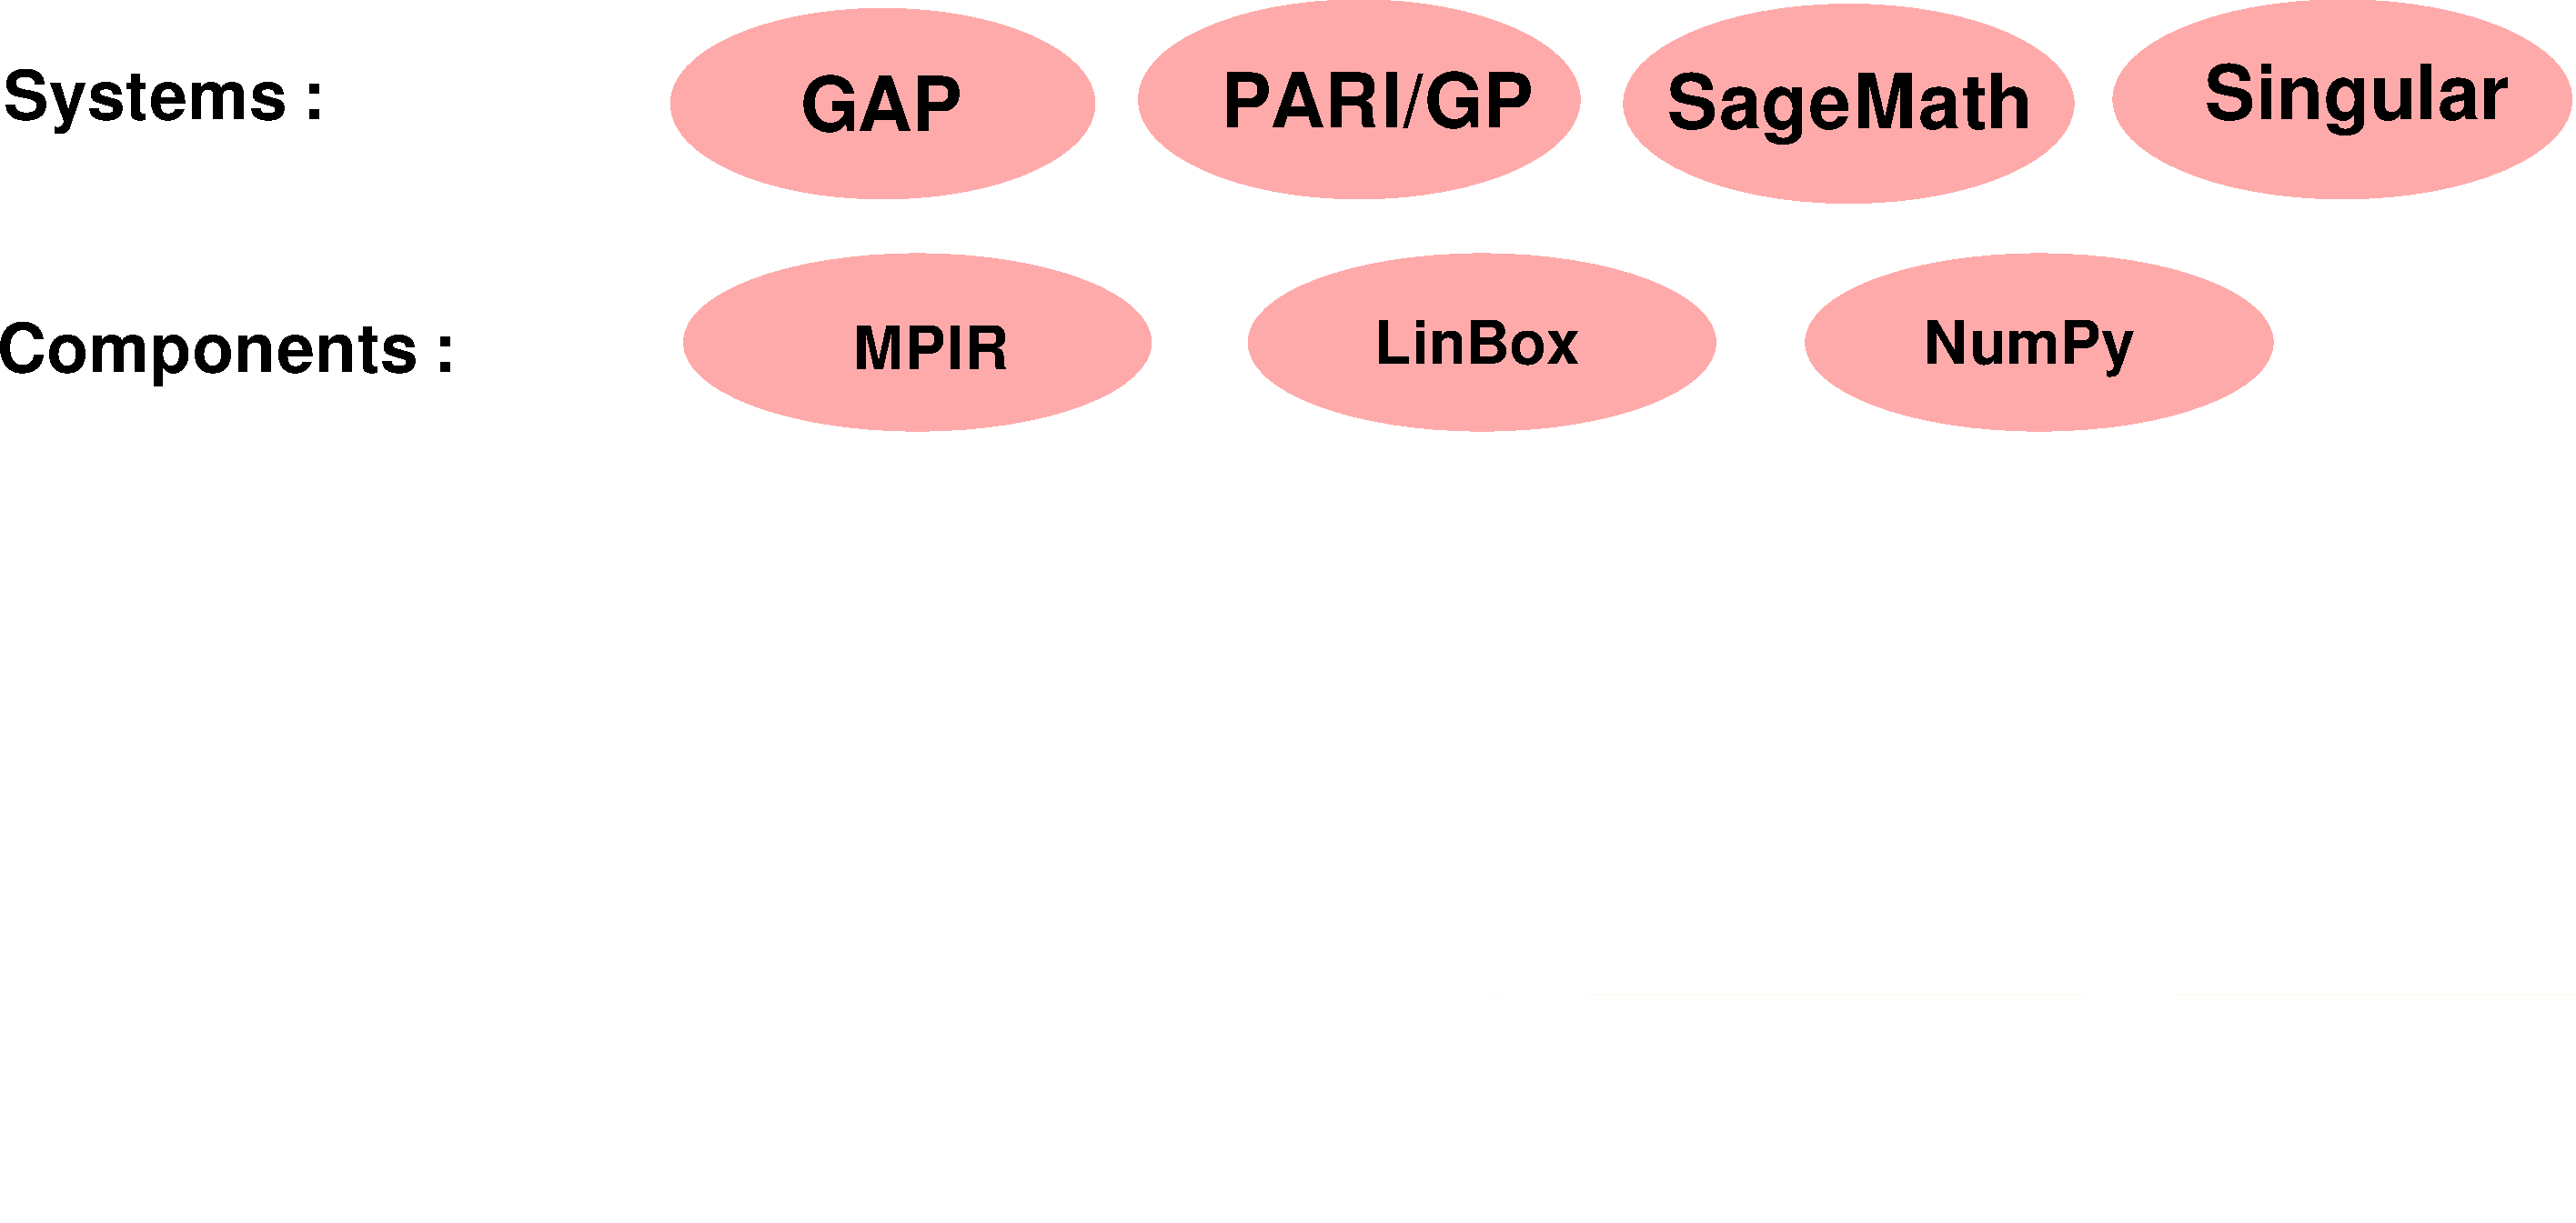
\includegraphics[width=0.8\textwidth]{software_stack_3}}

    \only<2>{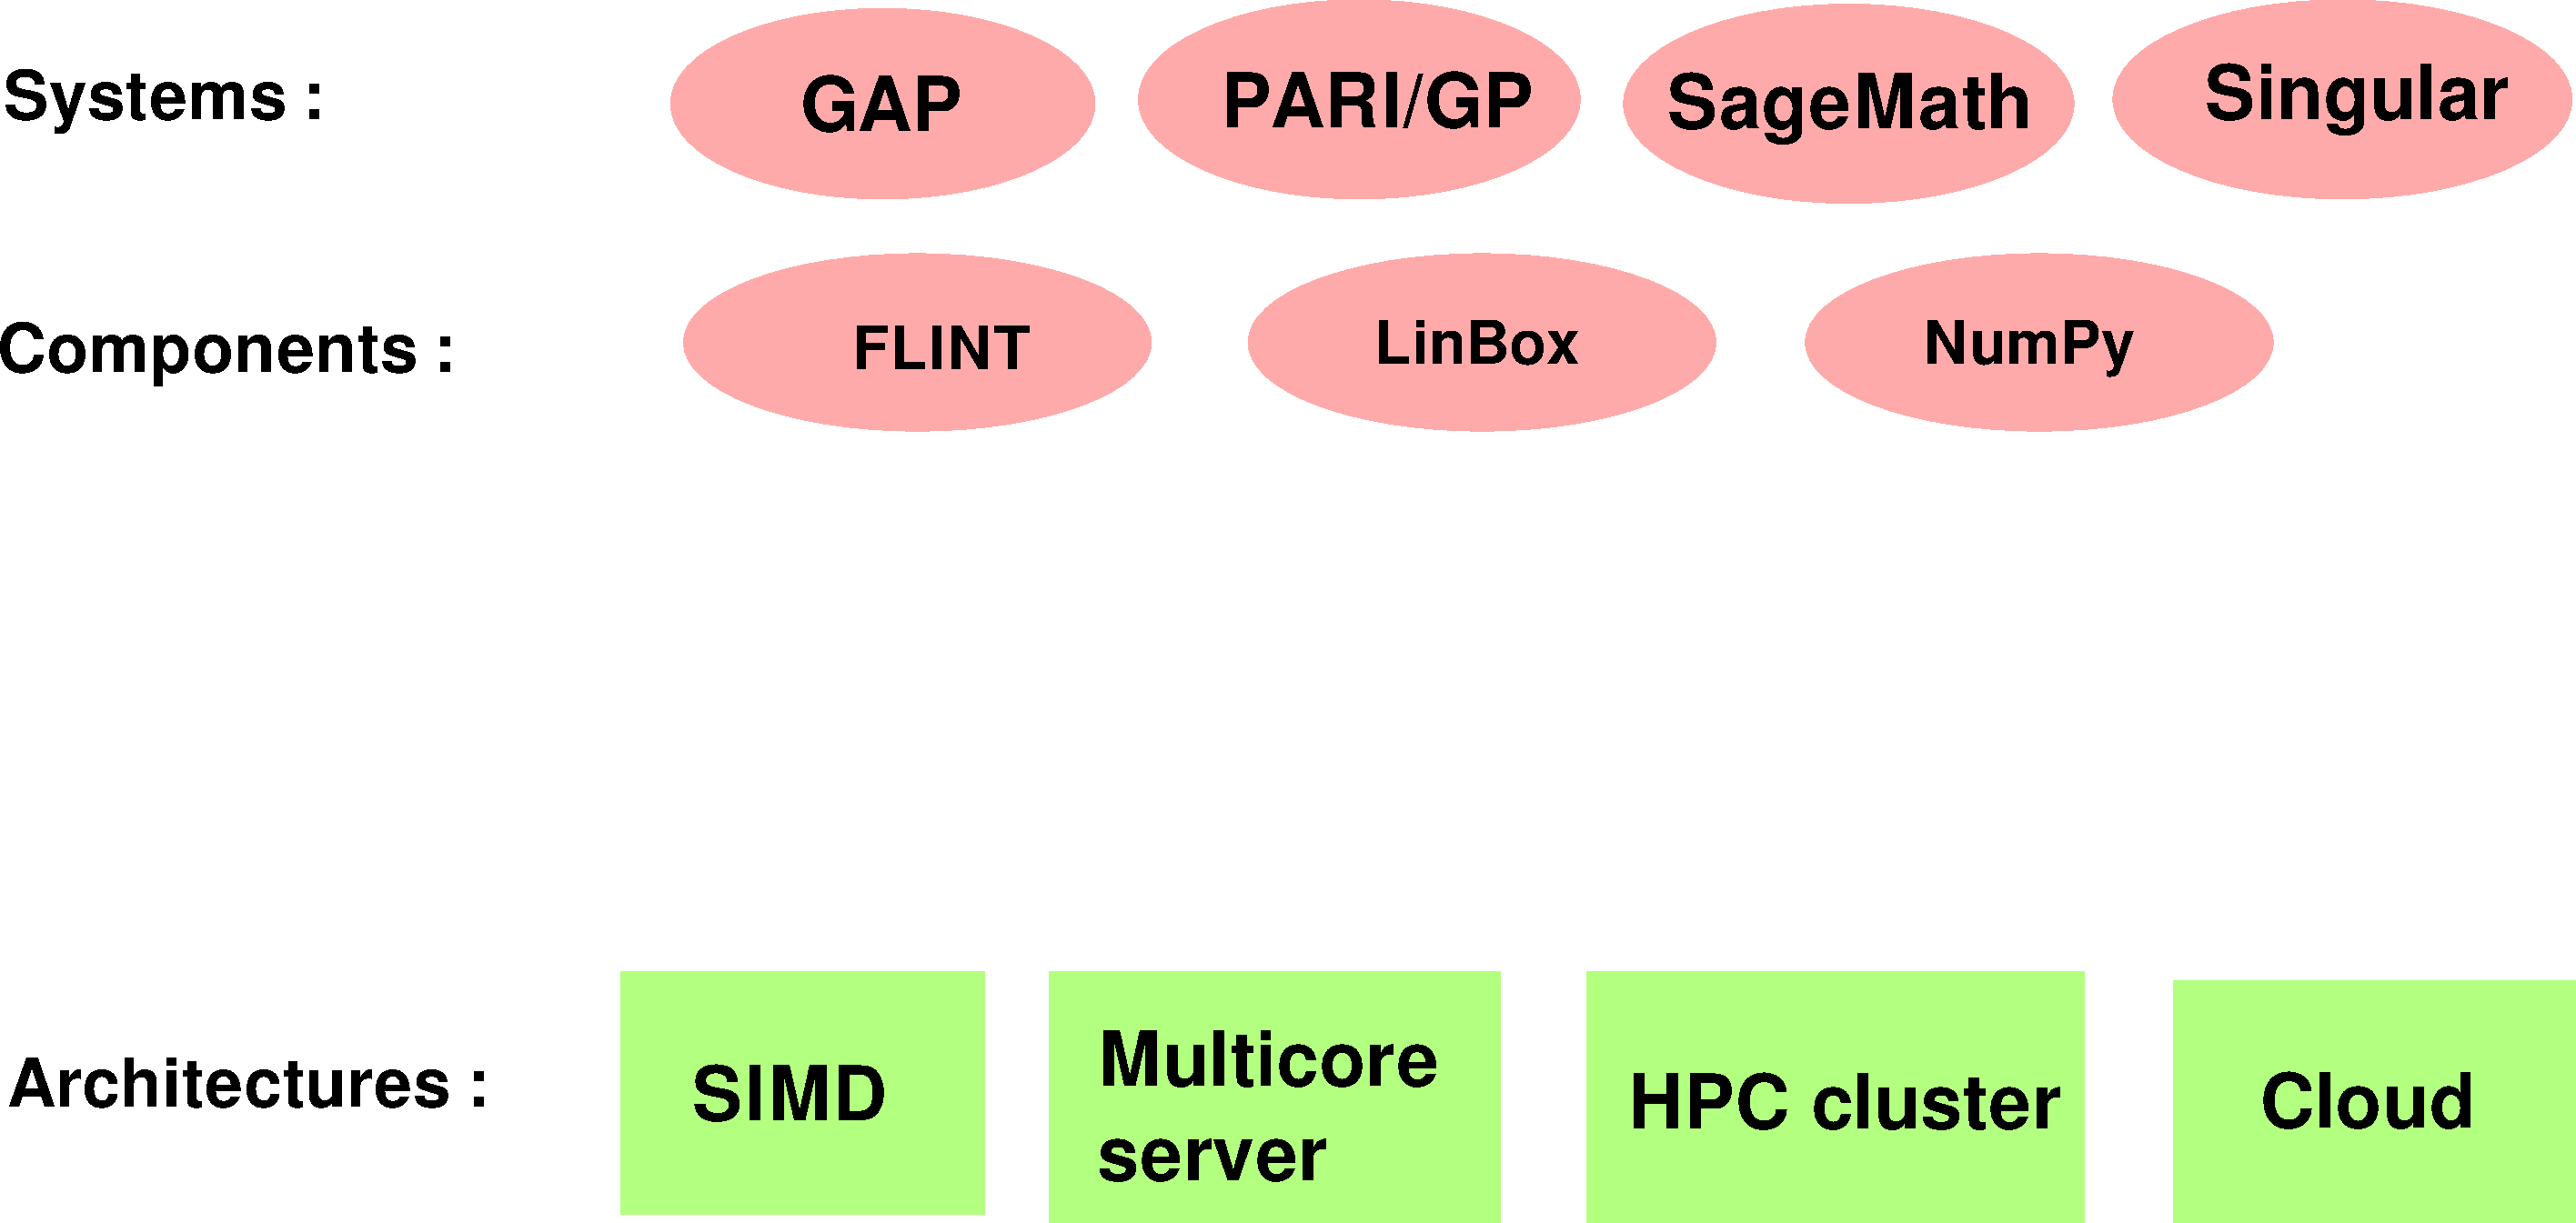
\includegraphics[width=0.8\textwidth]{software_stack_2}}
    
    \only<3>{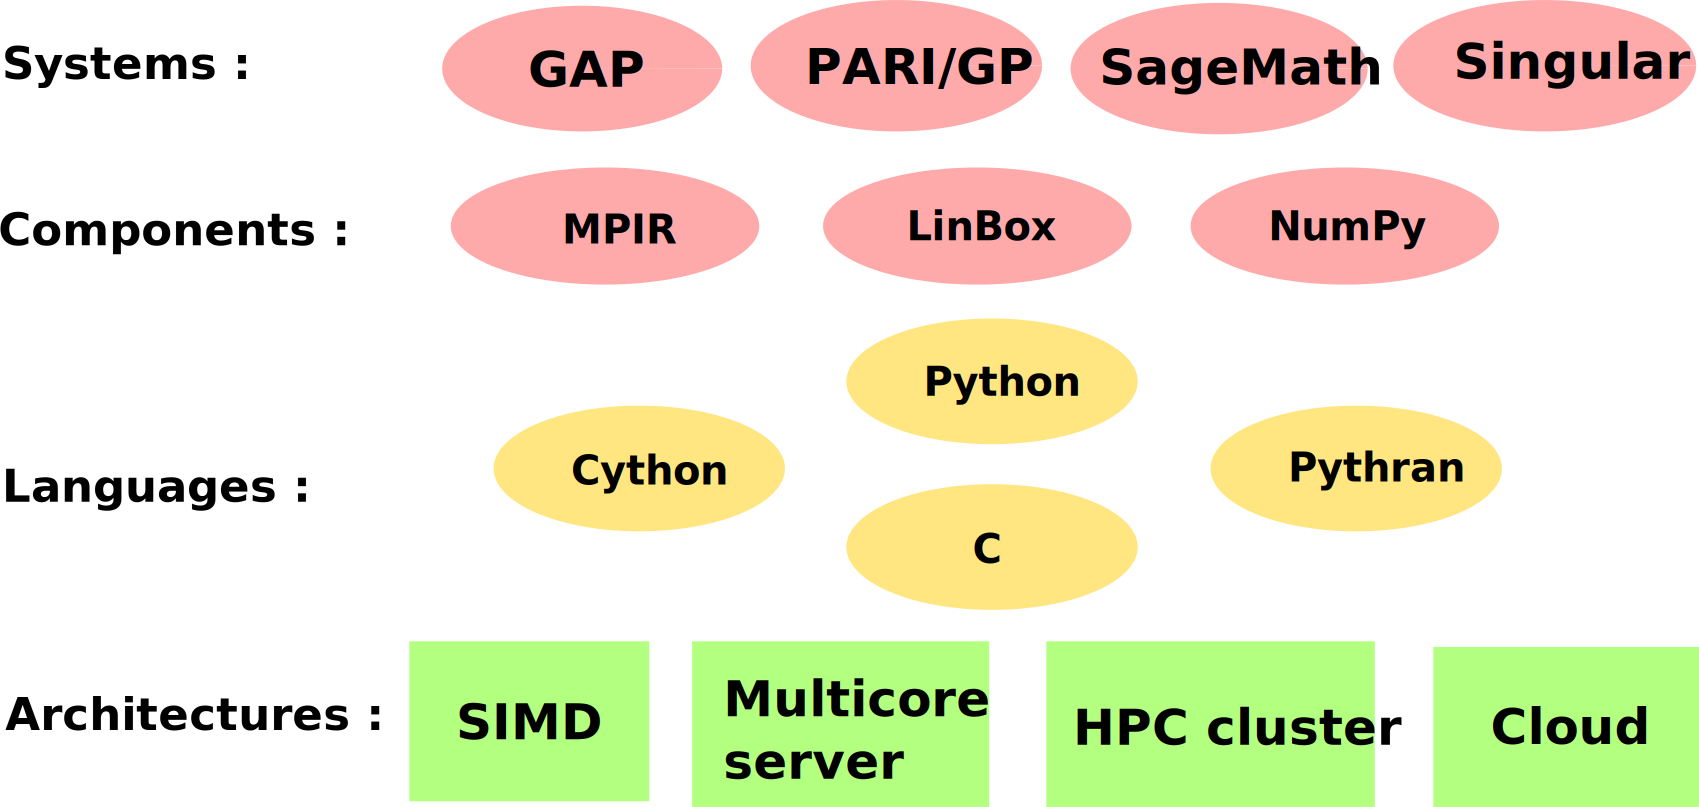
\includegraphics[width=0.8\textwidth]{software_stack}}

  \end{center}

\end{frame}
%%%%%%%%%%%%%%%%%%%%%%%%%%%%%%%%%%%%%%%%%%%%%%%%%%%%%%%%%
%% \begin{frame}
%%   \frametitle{Goal: delivering high performance to maths users}

%%     \begin{center}
%%     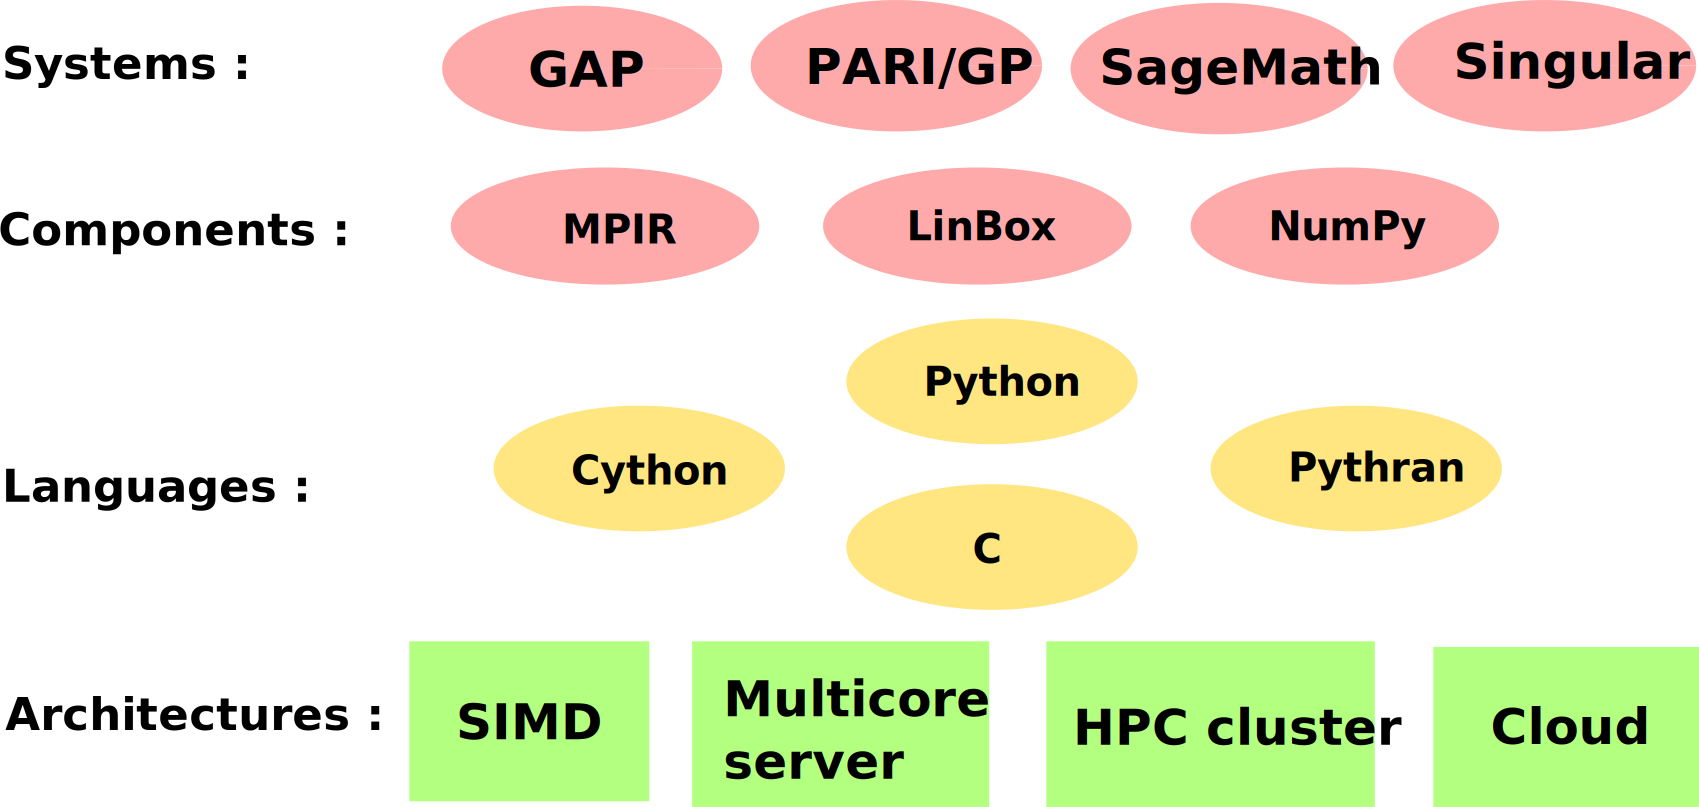
\includegraphics[width=0.8\textwidth]{software_stack}
%%   \end{center}

%%     \pause
%%     \begin{itemize}
%%     \item Improve/Develop parallel features of components first,
%%     \item Expose them through the software stack
%%     \item 
%%     \end{itemize}

%% \end{frame}


%%%%%%%%%%%%%%%%%%%%%%%%%%%%%%%%%%%%%%%
\begin{frame}
  \frametitle{High performance mathematical computing}
  \begin{block}
    {Goal:}
    \begin{itemize}
    \item Improve/Develop parallelization of software components
    \item Expose them through the software stack
    \item Offer High Performance Computing to VRE's users
    \end{itemize}
  \end{block}

  \begin{block}
      {Milestone M8: Seamless use of parallel computing architecture in the VRE (proof of concept)}

{\footnotesize  \textit{Astrid wants to run compute intensive routines involving both dense linear algebra and combinatorics. She has access through a JupyterHub-based VRE to a high end multi-core machine which includes a vanilla SAGE installation.
She automatically benefits from the HPC features of the underlying specialized
libraries (LinBox, ...). This is a proof of concept of the overall framework to
integrate the HPC advances of specialized libraries into a general purpose
VRE. It will prepare the final integration of a broader set of such parallel
features for the end of the project}
  }

  \end{block}
\end{frame}

%%%%%%%%%%%%%%%%%%%%%%%%%%%%%%%%%%%%%%%%%%%%%%%%%%%%%%

%% \begin{frame}[fragile]
%%   \frametitle{Milestone M8: Seamless use of parallel computing architecture in the VRE (proof of concept)}

%%   \begin{center}
%%     Live demo
%%   \end{center}
%% \end{frame}

%%%%%%%%%%%%%%%%%%%%%%%%%%%%%%%%%%%%%%%
%%%%%%%%%%%%%%%%%%%%%%%%%%%%%%%%%%%%%%%
%\section{Workpackage management}
\begin{frame}
  \frametitle{Outcome of WorkPackage 5}

  \begin{tabular}{lccc}
    \toprule
    Component & Review 1 & Review 2 & Final review\\
    \midrule
    T5.1 Pari/GP & & & {\color{green} D5.16} \\
    T5.2 GAP     & & & {\color{green} D5.15} \\
    T5.3 LinBox  & & \alert{D5.12} & {\color{green} D5.14} \\
    T5.4 Singular& D5.6, D5.7 & & {\color{green} D5.13} \\
    T5.5 MPIR    & D5.5, D5.7& & \\
    T5.6 Combinatorics  & D5.1& \alert{D5.11} & \\
    T5.7 Pythran        & D5.2 & \alert{D5.11} & \\
    T5.8 SunGrid Engine & D5.3 & & \\
    \bottomrule
    
  \end{tabular}

  \vspace{1em}
  
  Overall
  \begin{itemize}
  \item 31 software releases
  \item 16 research papers
  \end{itemize}
\end{frame}

%%%%%%%%%%%%%%%%%%%%%%%%%%%%%%%%%%%%%%%%%%%%%%%%%%%%%%
%%%%%%%%%%%%%%%%%%%%%%%%%%%%%%%%%%%%%%%
\begin{frame}  {Outline}
  \tableofcontents
\end{frame}



%%%%%%%%%%%%%%%%%%%%%%%%%%%%%%%%%%%%%%%%%%%%%%%%%%%%%%%%%%%%%
\section{Context and Focus}

  \begin{frame}
  \frametitle{Computational Kernels: linear algebra}
  \begin{displayquote}
    Mathematics is the art of reducing any problem to linear algebra\\
    \hfill{-- W. Stein}
  \end{displayquote}

\uncover<2->{  \begin{center}%
  \textbf{Linear algebra: a key building block for HPC}%
  \end{center}
  }
  \begin{block}<2-> {Similarities with numerical HPC}
    \begin{itemize}
    \item central elementary problem to which others reduce to
    \item (rather) simple algorithmic
    \item high compute/memory intensity
    \end{itemize}
  \end{block}
    \begin{block}<3->{Specificities}
      \begin{itemize}
      \item Multiprecision arithmetic $\Rightarrow$ lifting from finite  precision ($\mathbb{F}_p$)
      \item Rank deficiency $\Rightarrow$ unbalanced dynamic blocking
      \item Early adopter of subcubic matrix arithemtic $\Rightarrow$ recursion
      \end{itemize}
    \end{block}

  \end{frame}
  
  \begin{frame}
    \frametitle{Computational kernels: arithmetic}

    \begin{itemize}
    \item Wide variety of computing domains: $\Z,\Q,\Z/p\Z,\F_q, \F_q[X], \Z[X,Y,Z],..$
    \item possibly with dynamic size
    \end{itemize}

    \begin{block}{Challenge}
      \begin{itemize}
      \item most often memory intensive operations \thus hard to parallelize
      \item very fine grain, but billions of instance \thus fine tuning
      \end{itemize}
    \end{block}
  \end{frame}
  
%% %%%%%%%%%%%%%%%%%%%%%%%%%%%%%%%%%%%%%%%%%%%%%%%%%%%%%
%% \begin{frame}
%%   \frametitle{Libraries and systems}

%%   \begin{block} {Systems}
%%     \begin{itemize}
%%     \item GAP: huge code base, large contributed package collection
%%     \item PARI: 
%%     \end{itemize}
%%   \end{block}
%% \end{frame}
%%%%%%%%%%%%%%%%%%%%%%%%%%%%%%%%%%%%%%%%%%%%%%%%%%%%%%
%% \begin{frame}
%% \frametitle{Addressing recommendations of review 1}
%%     \textbf{Recommendation 10:} \textit{Regarding WP5, \textbf{make contacts} with HPC community in order to ascertain current state-of-the-art. The work in this WP needs to be \textbf{nearer the leading edge}.}

%%     \begin{description}
%%     \item<2-> [Leading edge achievements in linear algebra] \
%%       {\small
%%       \begin{itemize}
%%       \item symmetric factorization outperforms LAPACK implementation
%%       \item new non-hierarchical generator for quasiseparable matrices
%%       \item large scale parallelization of rational linear solver
%%       \end{itemize}
%%       }
%%     \begin{columns}
%%       \begin{column} {.3\textwidth}
%%         \begin{center}
%%           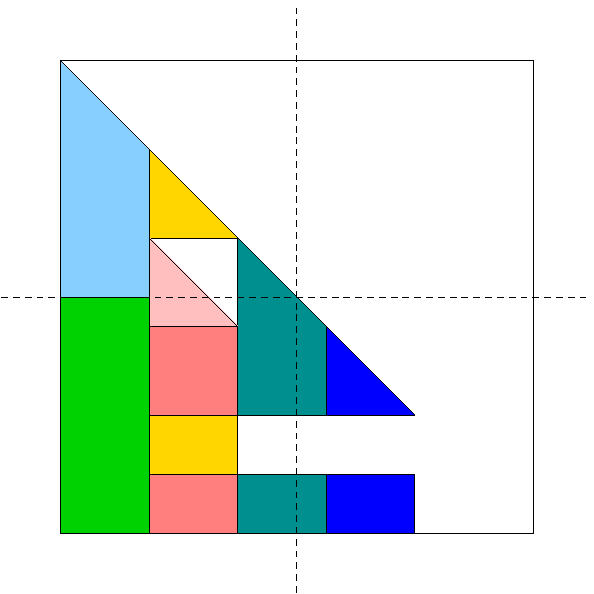
\includegraphics[width=.6\textwidth]{ARrec11}
%%       \end{center}
%%       \end{column}
%%       \begin{column} {.3\textwidth}
%%         \begin{center}
%%           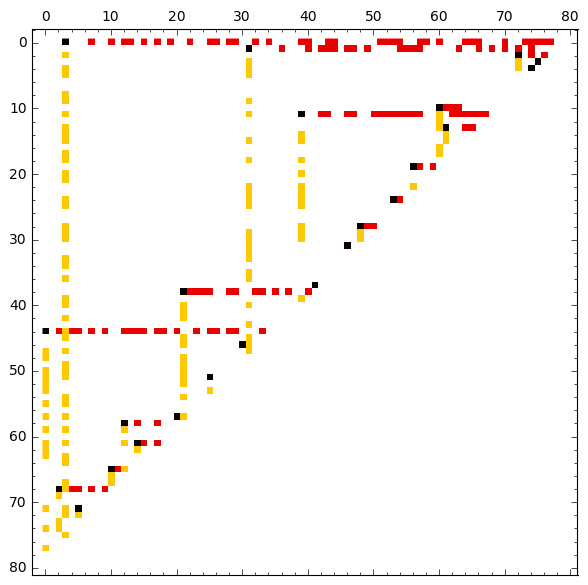
\includegraphics[width=.6\textwidth]{Bruhat}
%%         \end{center}
%%       \end{column}
%%       \begin{column} {.3\textwidth}
%%         \begin{center}
%%           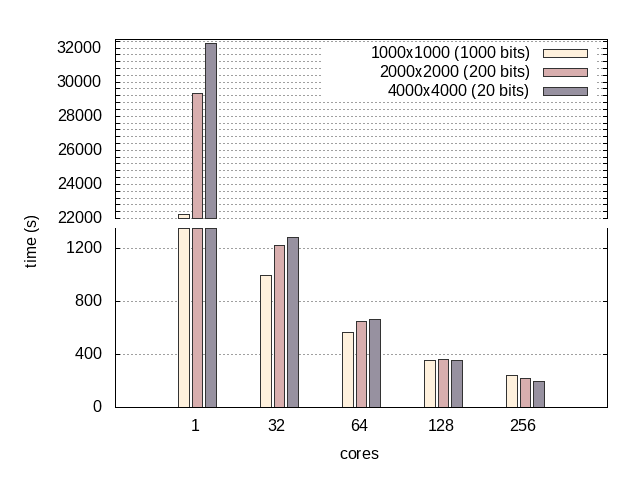
\includegraphics[width=.9\textwidth]{nodes_histogram}
%%         \end{center}
%%       \end{column}
%%     \end{columns}
%%     %% \item<3-> [Interactions and  contacts made:]\ 
%%     %%   {\small
%%     %%   \begin{itemize}
%%     %%   \item interaction with the \texttt{BLIS} group (vectorization and
%%     %%     implementation of Strassen's algorithm)
%%     %%   \item on-going collaboration with T. Mary (\texttt{Mumps}) and
%%     %%     S. Chandrasekaran (UCSB) on quasiseparable matrix algorithmic
%%     %%   \end{itemize}
%%     %%   }
%% \end{description}
%% \end{frame}


%%%%%%%%%%%%%%%%%%%%%%%%%%%%%%%%%%%%%%%
% TODO: should this be the same title as the one above
% "Addressing recommendations of review 1"
%% \begin{frame}
%%   \frametitle{Strengthening interactions with numerical HPC community}
%%   \begin{block}  {Existing connection}
%%     \begin{description}
%%     \item[Dense linear algebra] numerical BLAS used for exact FFLAS for 17 years
%%     \item[Pointwise interactions:] J. Dongarra, L. Grigori, J-Y. L'Excellent,  etc
%%     \item[Publications to main HPC venues:]
%%       SIAM-PPSC, EuroPar, PMAA, ParCo
%%     \item[Animation:] involved in the French CNRS \textit{Calcul}  working group (Sci. Comp.)
%%     \end{description}
%%   \end{block}
%%   \begin{block}<2->  {Recently established}
%%     \begin{itemize}
%%     \item With the \texttt{BLIS} group:
%%       \begin{itemize}
%%       \item Reporting bugs (SIMD vectorization)
%%       \item Sharing experience in implementing Strassen's algorithm
%%       \end{itemize}
%%     \item On-going collaboration with T. Mary (\texttt{Mumps}) and
%%         S. Chandrasekaran (UCSB) on quasiseparable matrix algorithmic
%%     \end{itemize}
%%   \end{block}
%% \end{frame}

%% %%%%%%%%%%%%%%%%%%%%%%%%%%%%%%%%%%%%%%%%%%%%%%%%%%%%%%%%%%%%%%%%%%%%%%%%%%%%%%
%%%%%%%%%%%%%%%%%%%%%%%%%%%%%%%%%%%%%%%%%%%%%%%%%%%%%%%%%%%%%%%%%%%%%%%%%%%%%%
\section{T5.1: Number theory with PARI/GP}
%%%%%%%%%%%%%%%%%%%%%%%%%%%%%%%%%%%%%%%%%%%%%%%%%%%%%%%%%%%%%%%%%%%%%%%%%%%%%%
%%%%%%%%%%%%%%%%%%%%%%%%%%%%%%%%%%%%%%%%%%%%%%%%%%%%%%%%%%%%%%%%%%%%%%%%%%%%%%
%% SLIDE 1: Main achievements (MT Engine)

%% We released a Multi-Thread engine for the complete PARI suite (Pari library,
%% GP shell, GP2C compiler). It supports
%% * Sequential computation,
%% * POSIX threads,
%% * Message Passing Interface (MPI),
%% within the same code base. The MT Engine is easy to setup
%% (Configure --mt=pthread, that's it). Part of it is transparent to users
%% (automatic implicit parallelism), part of it mirrors standard control
%% structures (for / parfor). [ Power users and developpers have complete
%% control on low-level aspects if they so desire. ]
\begin{frame}
  \frametitle{PARI-GP}

  \begin{block}
    {PARI ecosystem}

    \begin{description}
    \item[PARI library:] dedicated routines for number theory
    \item[PARI-GP:] an interactive system
    \item[GP2C:] a GP to C compiler
    \end{description}
  \end{block}
  \begin{block} {Generic parallelization engine for the whole suite}
    \begin{columns}
      \begin{column} {.44\textwidth}

    Delivers support for 
    \begin{itemize}
    \item sequential computations
    \item POSIX threads
    \item MPI for distributed computing
    \end{itemize}
      \end{column}
      \begin{column} {.55\textwidth}
        Features:
        \begin{itemize}
        \item Same code base
        \item automated parallelization
        \item full control for power users/developpers
        \end{itemize}
      \end{column}

    \end{columns}
  \end{block}
\end{frame}
%% SLIDE 2: Main achievements (libpari development)

%% * Fast linear algebra over the rationals and cyclotomic fields
%% * Fast Chinese remainders and multimodular reduction
%% * Parallel polynomial resultant [not yet quasi-linear]
%% * Fast modular polynomials and applications: ECPP primality proving, SEA
%% and Satoh point-counting
%% * MPQS integer factorization rewrite

%% Well-honed strategy after preliminary assessment:
%% * Improvement of code quality: refactoring, interface clarification
%% * Creation of "worker" functions from existing code
%% * Insertion of actual parallel instructions
%% [ Incremental buildup, independently instrumenting one high-level function at
%% a time. ]
\begin{frame} \frametitle{Main Achievements}
  \begin{itemize}
    \item  Fast linear algebra over the rationals and cyclotomic fields
    \item  Fast Chinese remainders and multimodular reduction
    \item Parallel polynomial resultant
    \item  Fast modular polynomials and applications%: ECPP primality proving, SEA and Satoh point-counting
     \item  MPQS integer factorization rewrite

  \end{itemize}
  \begin{block}   {Well-honed strategy after preliminary assessment}
    \begin{itemize}
%    \item Improvement of code quality: refactoring, interface clarification
    \item Creation of "worker" functions from existing code
    \item Insertion of actual parallel instructions
    \item Incremental buildup, independently instrumenting one high-level function at a time. 
    \end{itemize}
  \end{block}

  %% 
%% * 
\end{frame}
%% SLIDE 3: Highlight (Fast linear algebra)

%% Linear algebra over the rationals was a major bottleneck for independently
%% developped packages:
%% * Modular Symbols (2013-18)
%% * Modular Forms (2016-19).

%% These packages provided the main motivation and diverse testing grounds for
%% fast linear algebra using modular techniques, including but not limited to
%% parallelization:

%% * linear algebra over cyclotomic rings (Bill Allombert, 2016-17)
%% * fast multi-modular reduction and Chinese remainders (Bill Allombert, 2017)
%% * fast CUP decomposition over finite fields (Peter Bruin, 2018)
%% * parallelize through MT engine (Bill Allombert, Karim Belabas, 2017-19)


%% SLIDE 4: Highlight (Example of speedups)
\begin{frame}
  \frametitle{Highlight}

  \begin{columns}
    \begin{column}{.48\textwidth}
 Linear algebra over rationals:
 \begin{itemize}
  \item Required for cyclotomic rings (Allombert, 2016-17)
  \item Fast Chinese remaindering (Allombert, 2017)
  \item Fast CUP decomposition over finite fields (Bruin, 2018)
  \item Parallelization (Allombert, Belabas, 2017-19)
  \end{itemize}
    Fourier transform of $L$-functions
  
    \end{column}
    \begin{column}{.52\textwidth}
      \begin{center}

        \begin{tikzpicture}
\begin{axis}[
    title=Parallel speedup,
    xlabel={number of threads},
    ylabel={speedup},
    xmin=1, xmax=32,
    ymin=1, ymax=32,
    width=\textwidth
]
\addplot table {ellan-threads.dat};
  \addlegendentry{ellan}
\addplot table {matdet-threads.dat};
  \addlegendentry{matdet}
\addplot table {matker-threads.dat};
  \addlegendentry{matker}
\addplot [domain=0:32]{x}
         node [pos=0.6, sloped, above left]{ideal speedup};
\end{axis}
\end{tikzpicture}
  \end{center}   
    \end{column}
  \end{columns}
\end{frame}
% Using POSIX threads on a server with 8 physical cores (32 logical cores
%  through HyperThreading)

%% <picture, see attached image.tgz>

%% [ Compared to ellan, linear algebra involves more overhead: 3 atomic
%% parallelized operations (reducing inputs, modular linear algebra, Chinese
%% remaindering). In addition, matker wastes time in the main thread to check
%% the result. ]

%% SLIDE 5: Perspectives and new directions

%% In the continuity of ODK work:
%% * Parallelize MPQS integer factorization
%% [scheduled for end of year]
%% * Parallelize numerical summation and integration routines
%% [scheduled for 2020: not done yet because no impact outside of the
%% routine itself]
%% * Parallelize black-box linear algebra (block Lanczos or Wiedemann)
%% [scheduled for 2020: sequential code to be written first]

%% Outside of ODK scope: major projects that will both benefit from the newly
%% developped parallel code \emph{and} will themselves need to be parallelized
%% * Elliptic curve descent and prerequisite algebraic number theory (class
%% groups and units, compact units, principal ideal generators)
%% * Linear algebra over Z (HNF for class group computation)
%% [ Existing PARI or GP code already provides this, but in obscure or
%% inefficient ways. Major cleanup / overhaul needed. Can be done in an
%% incremental way, function by function. ]

%% old stuff
%% \begin{frame}
%%   \frametitle{T5.1: PARI}
%%   \begin{block} {D5.16: Pari Suite release, fully supporting parallelization}
%%     \begin{itemize}
%%     \item D5.10 (merged in D5.16):\\ Generic parallelization engine is now mature
%%       (released since Nov 2016). Support POSIX-threads and MPI.
%%     \item Current work: applying it throughout the library
%%       \begin{itemize}
%%       \item Chinese remaindering
%%       \item Rational linear algebra
%%       \item Discrete logarithm
%%       \item Resultants
%%       \item APRCL primality testing
%%       \end{itemize}
      
%%     \end{itemize}
%%   \end{block}
%% \end{frame}


%%%%%%%%%%%%%%%%%%%%%%%%%%%%%%%%%%%%%%%%%%%%%%%%%%%%%%%%%%%%%%%%%%%%%%%%%%%%%%
%%%%%%%%%%%%%%%%%%%%%%%%%%%%%%%%%%%%%%%%%%%%%%%%%%%%%%%%%%%%%%%%%%%%%%%%%%%%%%
\section{T5.2: Group theory with GAP}
%%%%%%%%%%%%%%%%%%%%%%%%%%%%%%%%%%%%%%%%%%%%%%%%%%%%%%%%%%%%%%%%%%%%%%%%%%%%%%
%%%%%%%%%%%%%%%%%%%%%%%%%%%%%%%%%%%%%%%%%%%%%%%%%%%%%%%%%%%%%%%%%%%%%%%%%%%%%%
%% \begin{frame}
%%   \frametitle{T5.2: GAP}
%%   \begin{block} {D5.15: Final report of GAP development}
%%     \begin{itemize}
%%     \item 8 releases were produced integrating contributions of D3.11 and D5.15
%%     \item Towards an integration of HPC-GAP: main release GAP-4.9
%%       \begin{itemize}
%%       \item Build system refactoring
%%       \item Ability to compile in HPC-GAP compatibility mode
%%       \end{itemize}
%%     \item Work in progress:
%%       \begin{itemize}
%%       \item  Multithreaded linear algebra: at the level of the \texttt{Meataxe} library
%%       \item Introspection functionalities: on-the-fly optimisation decision
%%       \end{itemize}
%%     \end{itemize}
%%   \end{block}
%% \end{frame}


\begin{frame}
  \frametitle{HPC GAP}

  \begin{columns}
    \begin{column}{.39\textwidth}
        \begin{block}{HPC-GAP}
          \begin{itemize}
          \item Multi-threaded GAP.
          \item Targets:
            \begin{itemize}
            \item multicore servers.
            \item good speedups
            \item high level abstraction
            \end{itemize}
            %    Flexible task farm; thread-safe data structures for the shared global knowledge pool; data race protection.
            %    Much of the library and some packages are now thread-safe
            %   Scaling is good 
          \end{itemize}
        \end{block}
    \end{column}
    
    \begin{column}{.59\textwidth}
      \begin{block} {Achievement}
        \begin{itemize}
        \item Fork from GAP,  diverged for a long time
        \item Huge effort to bring it back in:\\   GAP 4.9.1 (Month 33).\\
          \thus first GAP release with HPCGAP integrated as a compile-time option
        \end{itemize}
      \end{block}
    \end{column}
  \end{columns}

  \begin{center}
    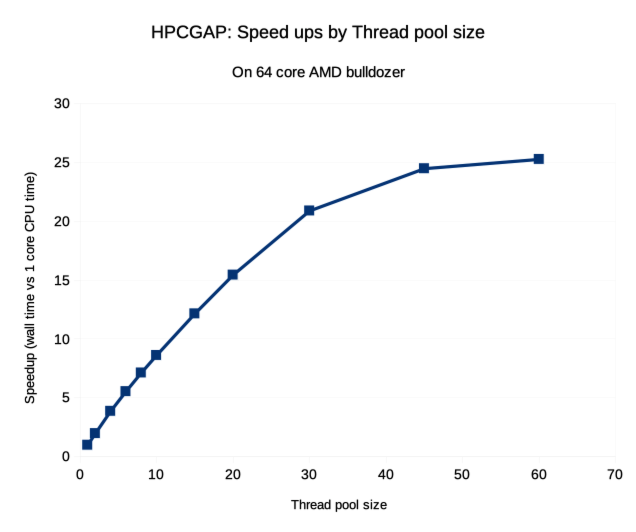
\includegraphics[height=.45\textheight]{hpcgap-speedups}
  \end{center}


\end{frame}
\begin{frame}
  \frametitle{Dense linear algebra over small finite fields}

  \begin{itemize}
  \item Matrix multiplication, Gaussian elimination, echelon forms, etc
  \item A key kernel for many GAP computations
  \end{itemize}

  \begin{block}{MeatAxe64}
  A new C and assembler library, tuned for performance at all levels:

  \begin{itemize}
  \item new data representations and assembler kernels
  \item new algorithms for many fields
  \item control of cache usage and memory bandwidth
    \thus allowing for sharing between threads and cores
  \item  purpose built highly efficient task farm

    \thus 1M x 1M dense matrix multiply over GF(2) in 8 hours (64 core AMD bulldozer).

  \end{itemize}
    Fully available from GAP.
  \end{block}

\end{frame}
%%%%%%%%%%%%%%%%%%%%%%%%%%%%%%%%%%%%%%%%%%%%%%%%%%%%%%%%%%%%%%%%%%%%%%%%%%%%%%
%%%%%%%%%%%%%%%%%%%%%%%%%%%%%%%%%%%%%%%%%%%%%%%%%%%%%%%%%%%%%%%%%%%%%%%%%%%%%%
\section{T5.3: Exact linear algebra with LinBox}
%%%%%%%%%%%%%%%%%%%%%%%%%%%%%%%%%%%%%%%%%%%%%%%%%%%%%%%%%%%%%%%%%%%%%%%%%%%%%%
%%%%%%%%%%%%%%%%%%%%%%%%%%%%%%%%%%%%%%%%%%%%%%%%%%%%%%%%%%%%%%%%%%%%%%%%%%%%%%



% TODO: too much text here! the second block is going out of the slide!
\begin{frame}
  \frametitle{Task 5.3: LinBox, High performance exact linear algebra}
  \begin{displayquote}
    Mathematics is the art of reducing any problem to linear algebra\\
    \hfill{-- W. Stein}
  \end{displayquote}

\uncover<2->{  \begin{center}%
  \textbf{Linear algebra: a key building block for HPC}%
  \end{center}
  }
  \begin{block}<2-> {Similarities with numerical HPC}
    \begin{itemize}
    \item central elementary problem to which others reduce to
    \item (rather) simple algorithmic
    \item high compute/memory intensity
    \end{itemize}
  \end{block}
    \begin{block}<3->{Specificities}
      \begin{itemize}
      \item Multiprecision arithmetic $\Rightarrow$ lifting from finite  precision ($\mathbb{F}_p$)
      \item Rank deficiency $\Rightarrow$ unbalanced dynamic blocking
      \item Early adopter of subcubic matrix arithemtic $\Rightarrow$ recursion
      \end{itemize}
    \end{block}
      
    \end{frame}

%%%%%%%%%%%%%%%%%%%%%%%%%%%%%%%%%%%%%%%%%%%%%%%%%%%%%%%%%%%%%%%%%%%%%%
\begin{frame}
  \frametitle{Parallel Rational solver algorithmic}
  \begin{center}
    \begin{tabular}{lc}
  \toprule
  Method  & Bit complexity \\
  \midrule
  Gauss over $\mathbb{Q}$ & $2^{\GO{n}}$ \\
  Gauss $\mod \text{bound}(sol)$ & $\GO{n^5}$\\
  Chinese Remaindering %CRT $\times$ Gauss $\mod p$
  & $\SO{n^4}
  $\\
  %\SO{n^{\omega+1}}$
  $p$-adic lifting & $\SO{n^3}$\\
  %, \SO{n^\omega}$\\
  \bottomrule
\end{tabular}
  \end{center}

  \begin{columns}
    \begin{column}{.48\textwidth}
      \begin{block}  {Chinese Remainder}
        \begin{enumerate}
        \item Solve the system independently modulo $p_1,p_2,\dots,p_k$
        \item Reconstruct a solution modulo $p_1\times p_2\times \dots,p_k$.
        \item Reconstruct over $\Q$
        \end{enumerate}
      \end{block}
    \end{column}
    \begin{column}{.48\textwidth}
      \begin{block} {$p$-adic lifting}
        \begin{enumerate}
        \item Solve the system modulo $p$
        \item Iteratively lift the solution modulo $p^2,p^3,\dots,p^k$
        \item Reconstruct over $\Q$
        \end{enumerate}
      \end{block}
    \end{column}
  \end{columns}
\end{frame}

%%%%%%%%%%%%%%%%%%%%%%%%%%%%%%%%%%%%%%%%%%%%%%%%%%%%%%%%%%%%%%%%%%%%%%
%%%%%%%%%%%%%%%%%%%%%%%%%%%%%%%%%%%%%%%%%%%%%%%%%%%%%%%%%%%%%%%%%%%%%%
%\subsection{Distributed memory Chinese remaindering}
\begin{frame}
  \frametitle{Distributed memory Chinese Remaindering}

      \begin{columns}
      \begin{column} {.5\textwidth}
        \begin{center}
          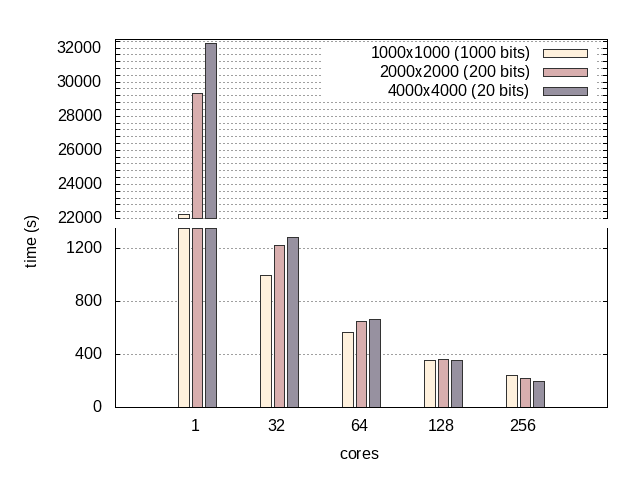
\includegraphics[width=\textwidth]{nodes_histogram}
      \end{center}
      \end{column}
      \begin{column} {.45\textwidth}
        \begin{center}
          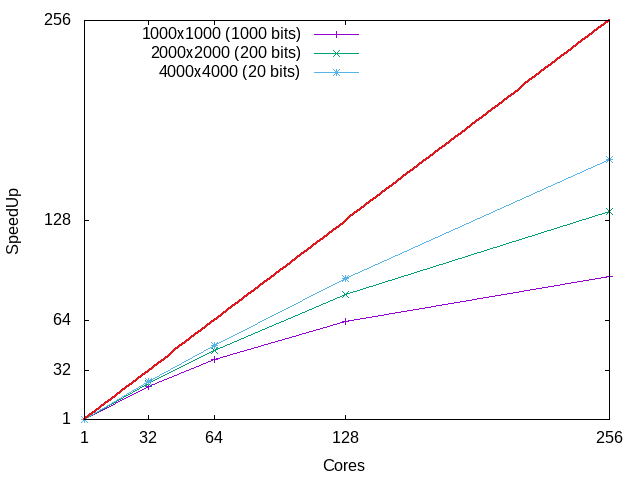
\includegraphics[width=\textwidth]{nodes_SPEEDUP}
        \end{center}
      \end{column}
      \end{columns}
      \begin{block}<1->{Conclusions}
        \begin{itemize}
        \item (almost) Embarrassingly parallel
        \item but overwhelming computational cost ($\SO{n^4}$)
        \item hybrid OpenMP-MPI version slightly slower but better memory efficiency
        \end{itemize}
      \end{block}
\end{frame}

%%%%%%%%%%%%%%%%%%%%%%%%%%%%%%%%%%%%%%%%%%%%%%%%%%%%%%%%%%%%%%%%%%%%%%
%%%%%%%%%%%%%%%%%%%%%%%%%%%%%%%%%%%%%%%%%%%%%%%%%%%%%%%%%%%%%%%%%%%%%%
%\subsection{Shared memory $p$-adic lifting}
\begin{frame}
  \frametitle{Shared memory $p$-adic lifting}

  \begin{block}    {A new hybrid algorithm:  Chinese Remaindering within $p$-adic lifting}
    \begin{itemize}
    \item Smaller critical path
    \item Higher degree of parallelism
    \end{itemize}
  \end{block}

    \begin{block}<2->{State of the art efficiency}
    \begin{columns}
      \begin{column}{.45\textwidth}
        \only<1,2>{
          Sequentially (1 thread):
        \begin{itemize}
        \item slight overhead
        \item amortized by a better memory access pattern (BLAS3)
        \item empirical setting of \# prime
        \end{itemize}
        }
        \only<3->{
          In parallel:
          \begin{itemize}
          \item Good scaling thanks to Chinese Remainder
          \item \# cores  \thus \# primes
          \end{itemize}
        }
      \end{column}
      \begin{column}{.53\textwidth}
        \only<1,2>{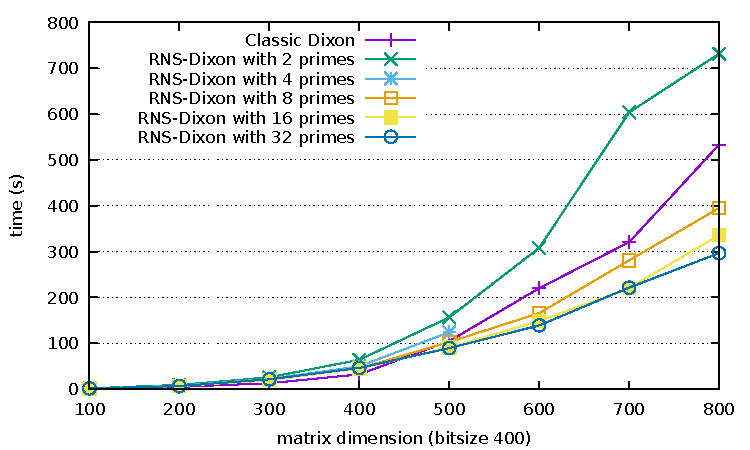
\includegraphics[width=1.03\textwidth]{sequential-primesCount}}

        \only<3->{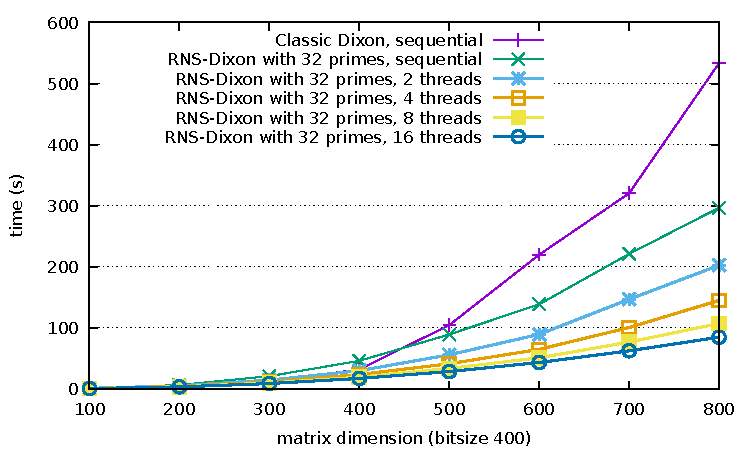
\includegraphics[width=1.03\textwidth]{parallel-threads}}
      \end{column}
    \end{columns}

  \end{block}
\end{frame}

%%%%%%%%%%%%%%%%%%%%%%%%%%%%%%%%%%%%%%%%%%%%%%%%%%%%%%%%%%%%%%%%%%%%%%
%\subsection{GPU enabled library}

%%%%%%%%%%%%%%%%%%%%%%%%%%%%%%%%%%%%%%%%%%%%%%%ù
\begin{frame}
  \frametitle{GPU enabled \texttt{fflas-ffpack}}
  \vspace{-1em}
  \begin{columns}
    \begin{column}{.62\textwidth}
      \begin{center}
        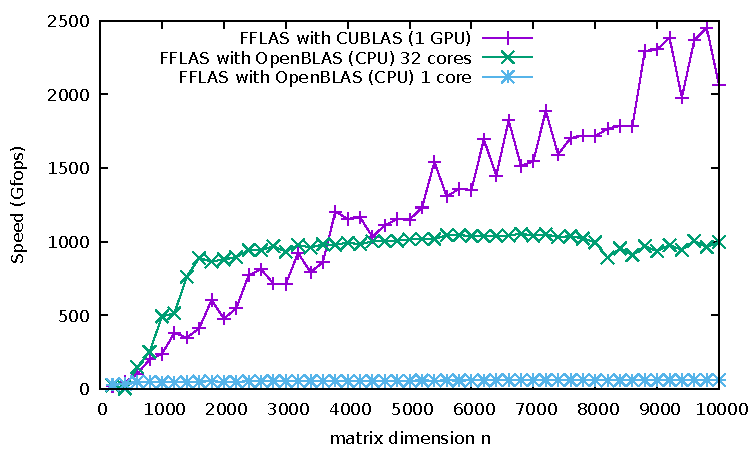
\includegraphics[width=\textwidth]{fgemm_GPUvsCPU}
      \end{center}
    \end{column}
    \begin{column}{.38\textwidth}
      \begin{itemize}
      \item Matrix product over $\Z/131071\Z$
      \item 32 Skylake-X cores (AVX512)
      \item 1 Nvidia Tesla V100 GPU
      \end{itemize}    
    \end{column}
  \end{columns}
%    \begin{figure}[H]
%      \caption{
      %}
      %   \end{figure}

      \begin{block}<2-> {Limitations and perspectives}
  \vspace{-1em}
        \begin{center}
        \alert{Bottleneck in the transfer between GPU and RAM}
        \end{center}
        \vspace{-1em}
        \begin{itemize}
        \item deport more computations to the GPU \hfill  \thus dedicated GPU kernels
        \item communication avoiding block scheduling \hfill \thus deep structural change
        \end{itemize}
      \end{block}
\end{frame}

%%%%%%%%%%%%%%%%%%%%%%%%%%%%
% TODO : a slide about LinBox' integration of these algs?
%%%%%%%%%%%%%%%%%%%%%%%%%%%%%%%%%%%%%%%%%%%%%%%%%%%%%%%

%% Old stuff

%%%%%%%%%%%%%%%%%%%%%%%%%%%%%%%%%%%%%%%
%\subsection{Exact linear algebra algorithms and implementations (D5.12).}


%% \begin{frame}
%%   \frametitle{D5.12: Exact linear algebra algorithms and implementations. Library maintenance and close integration in mathematical software for LinBox library}

%%   \begin{enumerate}
%%   \item Algorithmic innovations:
%%     \begin{enumerate}
%%     \item Rank deficient dense Gaussian elimination
%%     \item Quasiseparable matrices
%%     \item Outsourced computing security
%%     \end{enumerate}
%%   \item Software releases and integration:
%%     \begin{enumerate}
%%     \item LinBox ecosystem: \texttt{LinBox, fflas-ffpack, givaro}
%%     \item \texttt{SageMath} integration
%%     \end{enumerate}
%%   \end{enumerate}
%% \end{frame}

%% %%%%%%%%%%%%%%%%%%%%%%%%%%%%%%%%%%%%%%%
%% %% \begin{frame}
%% %%   \frametitle{Rank deficient dense Gaussian elimination}
%% %% %%   \begin{block}
%% %% %%     {[JSC'17] Fast computation of the rank profile matrix and the generalized
%% %% %%       Bruhat decomposition.}
%% %% %% {    \small
%% %% %%   \begin{itemize}
%% %% %%     \item Connecting Rank Profile Matrix and row and column echelon forms
%% %% %%     \item $O\tilde\ (r^\omega + mn)$ probabilistic time
%% %% %%     \item generalization over arbitrary rings
%% %% %%     \end{itemize}
%% %% %% }
%% %% %%   \end{block}

%% %%   \begin{block}{[ISSAC'18] Symmetric triangular factorization}
%% %%     \begin{columns}
%% %%       \begin{column} {.65\textwidth}
%% %%         \begin{itemize}
%% %%         \item First unconditional recursive algorithm
%% %%         \item Pivoting revealing the Rank Profile Matrix
%% %%         \item $O(n^2r^{\omega-2}) $ ($=1/3n^3$ with $\omega=3, r=n$)
%% %%         \item Also hot topic in numerical linear algebra \\ (LAPACK Working notes 294, Dec'17)
%% %%         \end{itemize}
%% %%       \end{column}
%% %%       \begin{column} {.25\textwidth}
%% %%         \begin{center}
%% %%           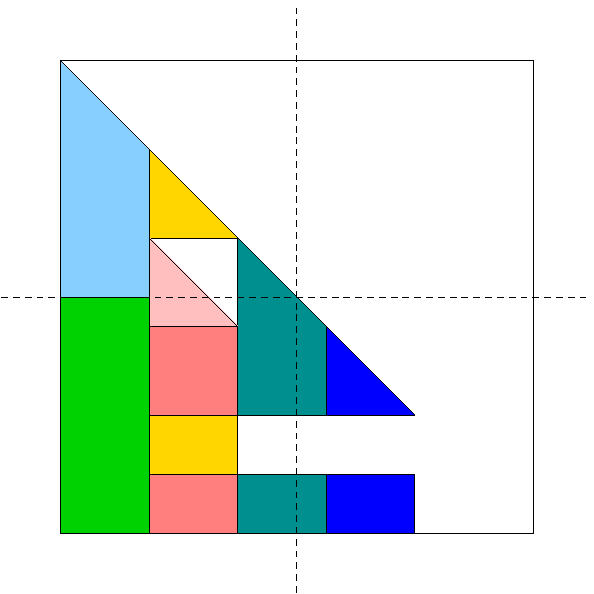
\includegraphics[width=\textwidth]{ARrec11}
%% %%         \end{center}
%% %%       \end{column}
%% %%     \end{columns}
%% %%   \end{block}
%% %% \end{frame}

%% %%%%%%%%%%%%%%%%%%%%%%%%%%%%%%%%%%%%%%%%%%%%%%%%%%%%%%%%%%%%%%%  
%% \begin{frame}[fragile]
%% \frametitle{LAPACK vs FFPACK modulo $8\,388\,593$}

%% {\footnotesize
%%   \begin{center}
%% \begin{tabular}{rrrrr}
%% \toprule
%% & \multicolumn{1}{c}{LAPACK (numerical)}&\multicolumn{1}{c}{FFPACK (exact)}\\
%% $n$ &  dsytrf (LDLT) & fsytrf (LDLT)\\
%% \midrule
%% 5000 & 1.60s  & \alert{1.59s} \\
%% 10000 & 11.98s &  \alert{10.90s} \\
%% \bottomrule
%% \end{tabular}
%% \end{center}
%% }
%% %\vspace{-5pt}
%% %\hspace{-20pt}
%% %\begin{minipage}{\textwidth}
%% \scriptsize
%% %\onslide+<2>
%% \begin{center}
%%   \begin{gnuplot}[terminal=cairolatex,terminaloptions={font ",10" linewidth 2}]
%%   set style line 3 pt 3 pi 50 lw 4 lt rgb "blue"
%%   set title 'Full rank, 1-core Intel Haswell i5-4690, \symbol{64}3.5GHz' offset 0,-0.75
%%   set ylabel 'Effective Gfops' offset 1,0
%%   set xlabel 'matrix dimension' offset 0,0.1
%%   set xtics rotate by 30 offset -2,-0.75
%%   set y2tics autofreq 
%%   set autoscale y2fixmin
%%   set autoscale y2fixmax  
%%   set size 0.8,0.75
%%   set key bottom right Left reverse
%%   plot [1:10000] [1:35] \
%%   "data_gflops.txt" using 1:3 title "LAPACK dsytrf" with lines lw 4 lc 2, \
%%   "data_gflops.txt" using 1:7 title "FFPACK fsytrf" with lines ls 3
%% \end{gnuplot}
%% \end{center}
%% %\end{minipage}
%% \end{frame}
%% %%%%%%%%%%%%%%%%%%%%%%%%%%%%%%%%%%%%%%%
%% %% \begin{frame}
%% %%   \frametitle{Quasiseparable matrices }
%% %%   \begin{center}
%% %%     \textit{Matrices with low off-diagonal rank}
%% %%   \end{center}

%% %%   \begin{block}
%% %%     {[ISSAC'16, JSC'18] New compact representation and algorithms}
%% %%   \begin{columns}
%% %%     \begin{column}{.75\textwidth}
%% %%     \begin{itemize}
%% %%     %\item Connection with rank profile matrix
%% %%     \item Matches the best space complexities%: $O(ns)$
%% %%     \item Reduction to matrix multiplication%: $O(ns^{\omega-1})$ for products
%% %%     \item \textbf{Breakthrough:} flat representation (non hierarchical)
%% %%     \end{itemize}
%% %%     \uncover<2->{
%% %%       \begin{description}
%% %%       \item[Follow-up:] on-going collaboration with numerical HPC experts:
%% %%         \begin{itemize}
%% %%         \item S. Chandrasekaran (UCSB)
%% %%         \item T. Mary (U. Manchester, \texttt{Mumps})
%% %%         \end{itemize}
%% %%       \end{description}
%% %%       }
%% %%     \end{column}
%% %%     \begin{column}{.2\textwidth}
%% %%       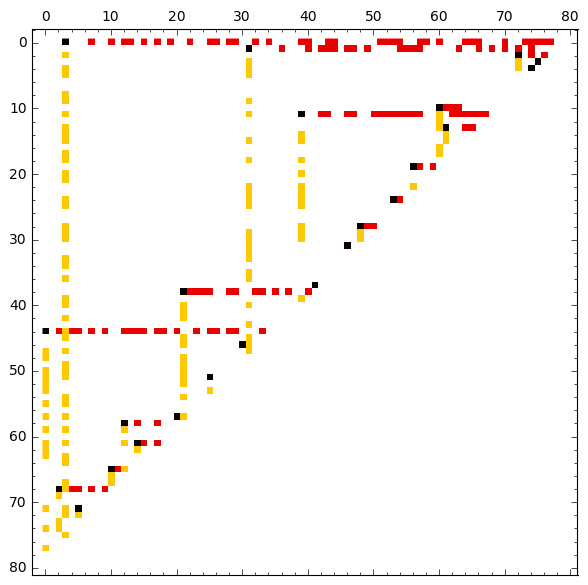
\includegraphics[width=\textwidth]{Bruhat}
%% %%     \end{column}
%% %%   \end{columns}
%% %%   \end{block}

%% %% \end{frame}


%% %%%%%%%%%%%%%%%%%%%%%%%%%%%%%%%%%%%%%%%
%% %%%%%%%%%%%%%%%%%%%%%%%%%%%%%%%%%%%%%%%%%%%%%%%%%%%%%%%%
%% \begin{frame}{Software releases and integration}
%%     \begin{block} {LinBox ecosystem}
%%       \begin{description}
%%         \item[\texttt{givaro}:] field/ring arithmetic
%%           \hfill{\uncover<2->{\alert{4 releases}}}
%%         \item[\texttt{fflas-ffpack}:] dense linear algebra over finite field \hfill{\uncover<2->{\alert{6 releases}}}
%%         \item[\texttt{LinBox}:] exact linear algebra \hfill{\uncover<2->{\alert{6 releases}}}
%%       \end{description}
%%       Tightly integrated  in \texttt{SageMath} \hfill{\uncover<2->{\alert{13 tickets}}}
%%     \end{block}

%%     \begin{block}<3-> {Featuring}
%%       \begin{itemize}
%%       \item Full functional implementations of new algorithmic contributions
%%       \item Improved vectorization and parallel routines
%%       \item Drastic improvement of reliability (continuous integration,
%%         test-suite coverage, randomized certificates, etc)
%%       \end{itemize}
%%     \end{block}
%% \end{frame}
%% %%%%%%%%%%%%%%%%%%%%%%%%%%%%%%%%%%%%%%%
%% \subsection{Distributed computing}
%% \begin{frame}
%%   \frametitle{Distributed computing  (on-going work)}

%%   \begin{block} {D5.14: Distributed exact linear system solving}
%% {
%%     \only<1,2>{
%%       \begin{itemize}
%%         \item 2 full time engineers
%%         \item Communication and serialization layer done
%%         \item Prototype MPI parallelization of Chinese remainder based solver.
%%       \end{itemize}
%%     }
%%     \only<3->{
%%       \begin{description}
%%       \item[Roadmap:] \
%%         \begin{itemize}
%%         \item Major refactorization of LinBox solver code under way
%%         \item Hybrid combination of CRT+Dixon and parallelization.
%%         \item Hyrbid OpenMP-MPI implementation
%%         \end{itemize}   
%%       \end{description}
%%         \vspace{-1.4em}
%%     }
%%     \begin{columns}
%%       \begin{column} {.5\textwidth}
%%         \begin{center}
%%           \uncover<2->{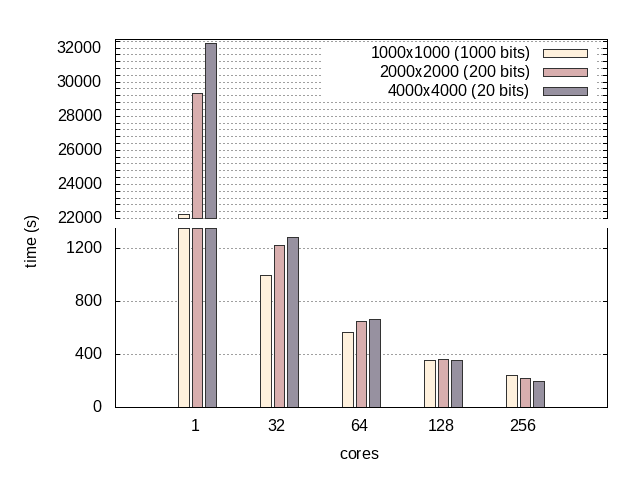
\includegraphics[width=\textwidth]{nodes_histogram}}
%%       \end{center}
%%       \end{column}
%%       \begin{column} {.45\textwidth}
%%         \begin{center}
%%           \uncover<2->{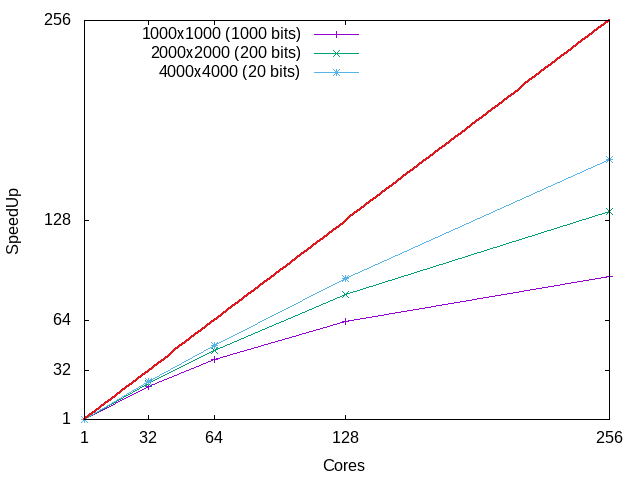
\includegraphics[width=\textwidth]{nodes_SPEEDUP}}
%%         \end{center}
%%       \end{column}
%%     \end{columns}
%% }
%%   \end{block}
%% \end{frame}

%%%%%%%%%%%%%%%%%%%%%%%%%%%%%%%%%%%%%%%%%%%%%%%%%%%%%%%%%%%%%%%%%%%%%%%%%%%%%%
%%%%%%%%%%%%%%%%%%%%%%%%%%%%%%%%%%%%%%%%%%%%%%%%%%%%%%%%%%%%%%%%%%%%%%%%%%%%%%
\section{T5.4: Polynomial arithmetic with Singular}
%%%%%%%%%%%%%%%%%%%%%%%%%%%%%%%%%%%%%%%%%%%%%%%%%%%%%%%%%%%%%%%%%%%%%%%%%%%%%%
%%%%%%%%%%%%%%%%%%%%%%%%%%%%%%%%%%%%%%%%%%%%%%%%%%%%%%%%%%%%%%%%%%%%%%%%%%%%%%


\frame{
\frametitle{Main achievements}

\begin{itemize}

\item Multivariate polynomials are in the \textsc{Flint} library over the coefficient rings $\mathbb{Z}$, $\mathbb{Q}$, $\mathbb{F}_p$, $\mathbb{F}_{p^n}$ for $p < 2^{64}$. The monomial orderings \emph{lex}, \emph{deglex}, and \emph{degrevlex} are currently supported. The computer algebra system \textsc{Singular} now uses \textsc{Flint} for multiplication, exact division, and gcd over $\mathbb{Q}$ and $\mathbb{F}_p$ for $p>500$.

\item The following operations are parallelized over $\mathbb{Z}$, $\mathbb{Q}$ and $\mathbb{F}_p$.
\begin{itemize}
\item multiplication
\item divisibility testing
\item greatest common divisor
\end{itemize}

\item The single-core algorithms are an improvement over the algorithms previously used in \textsc{Singular}.

\item The parallelism on large problems is 80\% to 90\% efficient on 8 threads and 70\% to 80\% efficient on 16 threads.

\item The library itself is well-tested and offers a consistent interface that allows it to be used for polynomial arithmetic in other computer algebra systems as well.

\end{itemize}

}

\frame{
\frametitle{New Perspectives}

\begin{itemize}

\item Though the single-core gains to arithmetic in \textsc{Singular} are real, the gains afforded by the thread-level parallelization of these operations are only applicable when the arithmetic operations are large.
\begin{itemize}
\item The process of splitting up the basic arithmetic task into independent tasks and combining the results is non-trivial and costs overhead.
\item Decent scaling of the multiplication to $16$ or $32$ threads requires huge polynomials.
\end{itemize}

\item Calculations that perform many arithmetic operations on small polynomials cannot expect to gain from our parallelization.
\begin{itemize}
\item These kind of calculations must and usually can benefit from parallelization at a higher level.
\end{itemize}

\item Multi-core timings are surprisingly fickle.
\begin{itemize}
\item Especially when \texttt{malloc} is involved - \texttt{malloc} is necessary because the sizes of the answer and the intermediate expressions in sparse polynomial arithmetic are completely unpredictable.
\item The fewer times \texttt{malloc} and \texttt{free} are called from a multi-threaded environment, the better!
\end{itemize}

\end{itemize}
}


\frame{
\frametitle{New Directions}

\begin{itemize}

\item Support for more monomial orderings
\begin{itemize}
\item Besides the commonly used orderings \emph{lexicographic}, \emph{graded lexicographic}, and \emph{graded reverse lexicographic}, other orderings such as block orderings and weighted orderings are possible and are used in \textsc{Singular}.
\item \textsc{Flint} is well-modularized and such orderings can be added once an interface is decided.
\item Such additions will not degrade the performance of the existing orderings.
\end{itemize}

\item Factorization
\begin{itemize}
\item Polynomial factorization is an important operation in many algorithms used in algebraic geometry.
\item Much of the infrastructure developed in \textsc{Flint} as part of ODK is directly applicable to factorization algorithms.
\item This would further improve the performance of \textsc{Singular}'s factorization, which is already quite good.
\end{itemize}

\end{itemize}

}




%%%%%%%%%%%%%%%%%%%%%%%%%%%%
%% % old stuff:
%% \begin{frame}
%%   \frametitle{T5.4 Singular}
%%   \begin{block}
%%     {D5.13: Parallel sparse polynomial multiplication}
    
%%     \texttt{FLINT} now supports fast sparse multivariate polynomials:
%%     \begin{itemize}
%%     \item addition, subtraction, multiplication,
%%     \item division, division with remainder, GCD
%%     \item evaluation, partial evaluation, composition
%%     \end{itemize}

%% \uncover<2->{  \textbf{Parallelization of the (sparse) multiplication}
%%     \begin{columns}
%%       \begin{column}{.4\textwidth}
%%         {\footnotesize
%%           %% \begin{equation*}
%%           %%   (1 + x + y + 2z^2 + 3t^3 + 5u^5)^{21}*(1 + u + t + 2z^2 + 3y^3 + 5x^5)^{21}
%%           %% \end{equation*}
%% %          \begin{center}
%%  %        \begin{center}
%%           \vspace{2mm}
          
%%           \begin{tabular}{lrr}
%%     \toprule
%%     \# & $\mathbb{Z}$ &  $\mathbb{Z}_{2^{64}-1}$  \\
%%     \midrule
%%    1 & 34145(1.0x) & 30349(1.0x) \\
%%    2 & 14856(2.3x) & 12641(2.4x) \\ 
%%    3 & 10844(3.1x) & 8294(3.6x)\\ 
%%    4 & 7205(4.7x) & 6274(4.8x) \\ 
%%    5 & 7621(4.4x) & 5315(5.7x) \\ 
%%    6 & 6156(5.5x) & 4152(7.3x) \\ 
%%    7 & 5679(6.0x) & 3739(8.1x) \\ 
%%    8 & 4458(7.6x) & 3047(9.9x) \\
%%    \bottomrule
%%   \end{tabular}
%%   %       \end{center}
%%          %% \begin{tabular}{lcccccccc}
%%  %%               \toprule
%%  %%               threads & time (ms) & speedup\\ \midrule
%%  %%               1 & 148661 & x1.0\\
%%  %%               2 & 76881 & x1.9\\ 
%%  %%               3 & 54798 & x2.7\\ 
%%  %%               4 & 42855 & x3.4\\ 
%%  %%               5 & 37017 & x4.0\\ 
%%  %%               6 & 30892 & x4.8\\ 
%%  %%               7 & 28365 & x5.2\\ 
%%  %%               8 & 28048 & x5.3\\
%%  %%               \bottomrule
%%  %%            \end{tabular}
%%  %% %       
%% %      \end{center}
%%         }
%%       \end{column}
%%       \begin{column}{.58\textwidth}
%%         \uncover<3->{
%%           \begin{itemize}
%%         \item Planned improvements to the memory manager $\Rightarrow$ closer to linear scaling 
%%         \item Parallel division and GCD implementations are in progress.
%%         \item Integration into Factory/Singular remains to be done
%%           \end{itemize}
%%           }
%%       \end{column}
%%     \end{columns}
%%     }
%%    \end{block}

%%  \end{frame}

%% \begin{frame}
%%   \frametitle{Root clustering}
    
%%     \begin{block}{Root clustering}
%% \begin{itemize}
%%  \item Remi Imbach has implemented the new parallel root clustering algorithm of Sagraloff-Yap
%%  \item Remi will return to Kaiserslautern (from New York visiting Chee Yap) to integrate the new code in Singular
%%  \item All deliverables for Kaiserslautern are on track
%%  \end{itemize}

%%  \end{block}
%%  \end{frame}

%%%%%%%%%%%%%%%%%%%%%%%%%%%%%%%%%%%%%%%%%%%%%%%%%%%%%%%%%%%%%%%%%%%%%%%%%%%%%%
%%%%%%%%%%%%%%%%%%%%%%%%%%%%%%%%%%%%%%%%%%%%%%%%%%%%%%%%%%%%%%%%%%%%%%%%%%%%%%
\begin{frame}
  \frametitle{Conclusion}

  \textbf{Outcome of WorkPackage 5}
  \begin{center}
{\small
    \begin{tabular}{lccc}
    \toprule
        & Review 1 & Review 2 & Final review\\
    \midrule
    T5.1 Pari/GP & & & {\color{darkgreen} D5.16} \\
    T5.2 GAP     & & & {\color{darkgreen} D5.15} \\
    T5.3 LinBox  & & {D5.12} & {\color{darkgreen} D5.14} \\
    T5.4 Singular& D5.6, D5.7 & & {\color{darkgreen} D5.13} \\
    T5.5 MPIR    & D5.5, D5.7& & \\
    T5.6 Combinatorics  & D5.1& {D5.11} & \\
    T5.7 Pythran        & D5.2 & {D5.11} & \\
    T5.8 SunGrid Engine & D5.3 & & \\
    \bottomrule
    
  \end{tabular}
}
  \end{center}
  
  Overall
  \begin{itemize}
  \item 31 software relases
    % 15 GAP
    % 3 PARI
    % 4 fflas
    % 2 givaro
    % 3 LinBox
    % 1 FLINT
    % 3 singular
  \item 16 research papers
  \end{itemize}
\end{frame}
  
%%%%%%%%%%%%%%%%%%%%%%%%%%%%%%%%%%%%%%%%%
\begin{frame}
  \frametitle{Lessons learnt}

  \begin{description}
    \item[From dedicated to general purpose HPC components:]\
      \begin{itemize}
      \item  Early instances of HPC computer algebra: dedicated to some target
        application (breaking RSA, etc)
      \item Building a general purpose HPC component:
        \begin{itemize}
        \item challenging
        \item longer term sustainability
        \end{itemize}
      \end{itemize}
    \item[Risk of technology dependency]\
      \begin{itemize}
      \item Cilk: from success to shut-down
      \item Interchangeability and modularity
      \end{itemize}
      \end{description}
  \end{frame}
%%%%%%%%%%%%%%%%%%%%%%%%%%%%%%%%%%%%%%%
\begin{frame} {Perspectives}

  \begin{block}{ Deployment of architecture dependent software stacks}
    \begin{itemize}
    \item dynamic runtime configuration\\
      \thus user decision based on algorithms (high level), not systems (low level)
      \thus compilation hurdle, vs slick interface of the VRE 
    \item extend high level control over parallel resources: GPUs, cluster nodes, etc

    \item keep as much HPC features as possible in  virtualization images
    \end{itemize}
  \end{block}
\end{frame}

%% \begin{frame}
%%   \frametitle{Extra Slides}

%%   \begin{center}
%%     \Large Extra Slides
%%   \end{center}
%% \end{frame}
%% \begin{frame}
%%   \frametitle{Outsourced computing security (D5.12)}

%%   \begin{block}{Exploratory aspect: Computation over the Cloud}
%%     \begin{description}
%%     \item[Outsourcing computation on the cloud:]\ 
%%       \begin{itemize}
%%       \item trusted lightweight client computer
%%       \item untrusted powerful cloud server
%%       \end{itemize}
%%       $\Rightarrow$ need for certification protocols
%%     \item[Multiparty computation:] \
%%       \begin{itemize}
%%       \item each player contribute with a share of the input
%%       \item shares must remain private
%%       \end{itemize}
%%     \end{description}
%% \end{block}
%%   \begin{block}<2->
%%       {Contribution}
%%       \begin{description}
%%         \item[ISSAC'17, JSC'19:] Linear time certificates for LU, Det., Rank Profile  matrix, etc
%%         \item[IWSEC'19:] Secure multiparty Strassen's algorithm
%%       \end{description}
%%   \end{block}

%% \end{frame}
%% %%%%%%%%%%%%%%%%%%%%%%%%%%%%%%%%%%%%%%%
%% \begin{frame}[fragile]{Exploration: Python, Cython, Pythran and Cilk (D5.8)}
%%   \textit{workshop: Interfacing (math) software with low level libraries}
%% \begin{center}
%%   \begin{gnuplot}[terminal=cairolatex,terminaloptions={font ",10" linewidth 2}]
%%   set style line 3 pt 3 pi 50 lw 4 lt rgb "blue"
%%   set title 'Counting descents in permutations'
%%   set logscale y
%%   set ylabel 'log time'
%%   set format y '%L'
%%   set xlabel 'n'
%%   set size 0.9,0.6
%%   set key bottom right
%%   plot [9:13] \
%%   "data_perms.txt" using 1:2 title "python" with lines lc 1, \
%%   "data_perms.txt" using 1:4 title "cython/pythran" with lines lc 3, \
%%   "data_perms.txt" using 1:6 title "cilk 1 core" with lines lc 5, \
%%   "data_perms.txt" using 1:7 title "cilk 8 cores" with lines lc 6
%%   \end{gnuplot}

%% \begin{itemize}
%% \item Python (interpreted language) slow.
%% \item Cython/Pythran (Python to C compilers) efficient.
%% \item Cilk (SIMD and multithread parallelism) very promising.
%% \end{itemize}
%% \end{center}

%% \end{frame}
%%%%%%%%%%%%%%%%%%%%%%%%%%%%%%%%%%%%%%%
%%%%%%%%%%%%%%%%%%%%%%%%%%%%%%%%%%%%%%%
\end{document}
